\documentclass[tikz, border=15pt]{standalone}
\usepackage{tikz}
\usetikzlibrary{positioning, calc}

\begin{document}

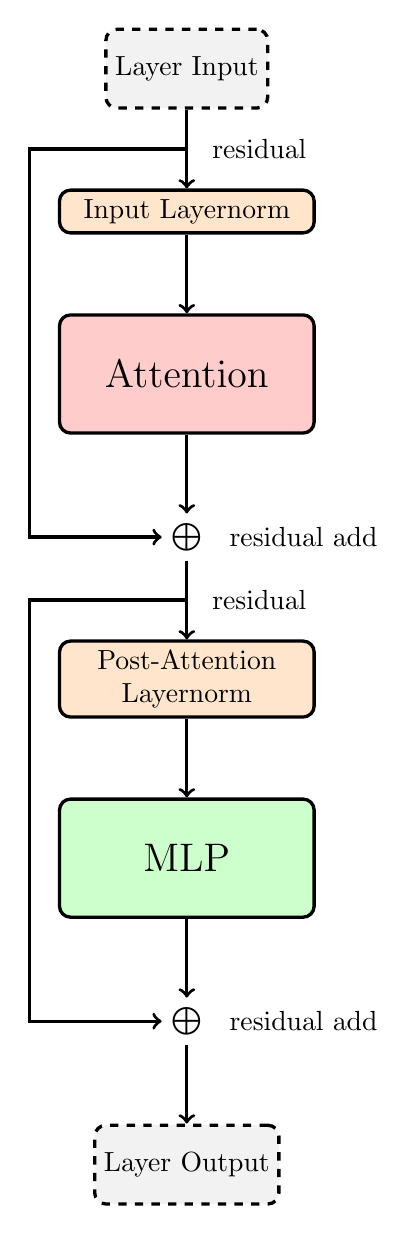
\begin{tikzpicture}[
    data/.style={
        draw,
        very thick,
        rounded corners,
        minimum width=2cm,
        minimum height=1cm,
        dashed,
        fill=gray!10, 
    },
    module/.style={
        draw,
        very thick,
        rounded corners,
        minimum width=2cm,
        minimum height=1.5cm,
        text width=3cm,
        align=center,
        font=\Large,
    },
    norm/.style={
        draw,
        very thick,
        rounded corners,
        minimum width=2cm,
        text width=3cm,
        align=center,
        fill=orange!20,
    },
    arrow/.style={
        ->,
        very thick,
    },
]

    \node[data] (inp) {Layer Input};
    \coordinate[below=0.5 cm of inp] (split1);
    \node[right=0.2 cm of split1] (res1) {residual};
    \coordinate[left=2 cm of split1] (split1_left);
    \node[norm, below=0.5 cm of split1] (norm1) {Input Layernorm};
    \node[module, below=of norm1, fill=red!20] (attn) {Attention};
    \node[below=of attn] (add1) {$\bigoplus$};
    \node[right=0.1 cm of add1] (res1_add) {residual add};
    \coordinate[below=0.5 cm of add1] (split2);
    \node[right=0.2 cm of split2] (res2) {residual};
    \coordinate[left=2 cm of split2] (split2_left);
    \node[norm, below=0.5 cm of split2] (norm2) {Post-Attention Layernorm};
    \node[module, below=of norm2, fill=green!20] (mlp) {MLP};
    \node[below=of mlp] (add2) {$\bigoplus$};
    \node[right=0.1 cm of add2] (res2_add) {residual add};
    \node[data, below=of add2] (out) {Layer Output};

    % Draw arrows
    \draw[arrow] (inp) -- (norm1);
    \draw[arrow] (split1) -- (split1_left) |- (add1);
    \draw[arrow] (norm1) -- (attn);
    \draw[arrow] (attn) -- (add1);
    \draw[arrow] (add1) -- (norm2);
    \draw[arrow] (split2) -- (split2_left) |- (add2); 
    \draw[arrow] (norm2) -- (mlp);
    \draw[arrow] (mlp) -- (add2);
    \draw[arrow] (add2) -- (out);

\end{tikzpicture}

\end{document}